\documentclass{article}

\setlength{\headsep}{0.75 in}
\setlength{\parindent}{0 in}
\setlength{\parskip}{0.1 in}

%=====================================================
% Add PACKAGES Here (You typically would not need to):
%=====================================================

\usepackage[margin=1in]{geometry}
\usepackage{amsmath,amsthm}
\usepackage{fancyhdr}
\usepackage{enumitem}
\usepackage{graphicx}
%=====================================================
% Ignore This Part (But Do NOT Delete It:)
%=====================================================

\theoremstyle{definition}
\newtheorem{problem}{Problem}
\newtheorem*{fun}{Fun with Algorithms}
\newtheorem*{challenge}{Challenge Yourself}
\def\fline{\rule{0.75\linewidth}{0.5pt}}
\newcommand{\finishline}{\vspace{-15pt}\begin{center}\fline\end{center}}
\newtheorem*{solution*}{Solution}
\newenvironment{solution}{\begin{solution*}}{{} \end{solution*}}
\newcommand{\grade}[1]{\hfill{\textbf{($\mathbf{#1}$ points)}}}
\newcommand{\thisdate}{\today}
\newcommand{\thissemester}{\textbf{Rutgers: Spring 2021}}
\newcommand{\thiscourse}{CS 344: Design and Analysis of Computer Algorithms} 
\newcommand{\thishomework}{Number} 
\newcommand{\thisname}{Name} 
\newcommand{\thisextension}{Yes/No} 

\headheight 40pt              
\headsep 20pt
\renewcommand{\headrulewidth}{0pt}
\lhead{\small \textbf{Only for the personal use of students registered in CS 344, Spring 2021 at Rutgers University. Redistribution out of this class is strictly prohibited.}}
\pagestyle{fancy}

\newcommand{\thisheading}{
   \noindent
   \begin{center}
   \framebox{
      \vbox{\vspace{2mm}
    \hbox to 6.28in { \textbf{\thiscourse \hfill \thissemester} }
       \vspace{8mm}
       \hbox to 6.28in { {\Large \hfill  Midterm Exam \#\thishomework \hfill} }
       \vspace{2mm}
         \hbox to 6.28in { {\hfill Due: Tuesday, March 2nd, 9:00am EST \hfill} }
       \vspace{4mm}
       \hbox to 6.28in { \emph{Name: \thisname \hfill NetID: \thisextension}}
      \vspace{2mm}}
      }
   \end{center}
   \bigskip
}

%=====================================================
% Some useful MACROS (you can define your own in the same exact way also)
%=====================================================


\newcommand{\ceil}[1]{{\left\lceil{#1}\right\rceil}}
\newcommand{\floor}[1]{{\left\lfloor{#1}\right\rfloor}}
\newcommand{\prob}[1]{\Pr\paren{#1}}
\newcommand{\expect}[1]{\Exp\bracket{#1}}
\newcommand{\var}[1]{\textnormal{Var}\bracket{#1}}
\newcommand{\set}[1]{\ensuremath{\left\{ #1 \right\}}}
\newcommand{\poly}{\mbox{\rm poly}}

\newcommand{\leasttwoalg}{\textnormal{\texttt{FIND-SMALLEST-TWO}}}
\newcommand{\totalsum}{\textnormal{\texttt{TOTAL-SUM}}}
\newcommand{\maxalg}{\textnormal{\texttt{MAX-ALG}}}
\newcommand{\minalg}{\textnormal{\texttt{MIN-RAND-ALG}}}

%=====================================================
% Fill Out This Part With Your Own Information:
%=====================================================


\renewcommand{\thishomework}{1} %Homework number
\renewcommand{\thisname}{Letao Zhang} % Your name
\renewcommand{\thisextension}{186004459} % Pick only one of the two options accordingly

\begin{document}

\thisheading

\vspace{-0.5cm}
\subsection*{Instructions}

\begin{enumerate}
	\item Do not forget to write your name and NetID above, and to sign Rutgers honor pledge below. 
	\item The exam contains $5$ problems worth $100$ points in total \emph{plus} one {extra} credit problem worth $10$ points. 
	\item This is a take-home exam. You have until Tuesday, March 2nd, 9:00am EST to finish the exam. 
	\item The exam should be done \textbf{individually} and you are not allowed to discuss these questions with anyone. This includes asking any questions or clarifications
	regarding the exam from other students or posting them publicly on Piazza (any inquiry should be sent directly to the Instructor or posted privately on Piazza). You may however consult all
	the materials used in this course (video lectures, notes, textbook, etc.) while writing your solution, but \textbf{no other resources are allowed}.

	\item Remember that you can leave a problem (or parts of it) entirely blank and receive $25\%$ of the grade for that problem (or part). However, this should not  discourage you from attempting a problem if you think 
	you know how to approach it as you will receive partial credit more than $25\%$ as long as you are on the right track. But keep in mind that if you simply do not know the answer, writing a totally wrong answer may lead to $0\%$ credit.
	
	The only \textbf{exception} to this rule is the extra credit problem: you do {not get any credit for leaving the extra credit problem blank}, and it is harder to get partial credit on that problem.
	
	\item \textbf{You should always prove the correctness of your algorithm and analyze its runtime.} Also, as a general rule, avoid using complicated pseudo-code and instead explain your algorithm in English. 
	\item You may use any algorithm presented in the class or homeworks as a building block for your solutions. 
\end{enumerate}

\finishline

\paragraph{Rutgers honor pledge:} Please sign the Rutgers honor pledge below. 

\begin{quote}
\emph{On my honor, I have neither received nor given any unauthorized assistance on this
examination.} 
\end{quote}
\hfill{Signature:\underline{Letao Zhang}}

\bigskip

\begin{center}
\begin{tabular}{|c|r|c|}
\hline
Problem. \# & Points & Score \\ \hline\hline
$1$ & 20 & ~~~~~~~~~~~\\  \hline
$2$ & 20 & \\ \hline
$3$ & 20 & \\ \hline
$4$ & 20 & \\ \hline
$5$ & 20 & \\ \hline
$6$ & +10 & \\ \hline
Total & $100 + 10$ & \\ \hline
\end{tabular}
\end{center}

\newpage

\begin{problem}\label{basics}~
\begin{enumerate}[label=(\alph*)]
	\item Determine the \emph{strongest} asymptotic relation between the functions 
	\[
	f(n) = \sqrt{\log{n}} \quad \text{and} \quad g(n) = \frac{n}{2^{(\log\log{n})}},
	\]
	i.e., whether $f(n) = o(g(n))$, $f(n) = O(g(n))$, $f(n) = \Omega(g(n))$, $f(n) = \omega(g(n))$, or $f(n) = \Theta(g(n))$. 
	Remember to prove the correctness of your choice. \grade{10}

\bigskip
\begin{solution}
	
	$\frac{n}{2^{(\log\log{n})}} = \Omega( \sqrt{\log{n}})$. \\
	
	We firstly simplify both equations by multiplying log that $f(n) = \sqrt{\log{n}} = \log{\sqrt{\log{n}}} = \frac{1}{2}\log(\log{n})$. \\
	
	$g(n) = \frac{n}{2^{(\log\log{n})}} = \log{\frac{n}{2^{(\log\log{n})}}}= \log{n} - \log{2^{(\log\log{n})}} = \log{n} - \log\log{n}\log_22 = \log{n} - \log\log{n}$. \\
	
	Then, we know that  $\log{n} \geq \log\log{n}$. We thus have $g(n) = \log{n}$. \\
	
	Therefore, $f(n) \leq g(n)$. For 	\emph{lower bound}, we get that $\lim_{n \to \infty}\frac{\log{n}}{1/2\log\log{n}} = \infty$. Thus, $\frac{n}{2^{(\log\log{n})}} = \Omega( \sqrt{\log{n}})$. \\
	
\end{solution}

	\newpage
	\item Use the \emph{recursion tree} method to solve the following recurrence $T(n)$ by finding the \emph{tightest} function $f(n)$ such that $T(n) = O(f(n))$:   \grade{10}
	\begin{align*}
		T(n) &\leq 8 \cdot T(n/2) + O(n^3). 
	\end{align*} 
	(You do \emph{not} have to prove that your function is the tightest one.) 
	\bigskip
	\begin{solution}
	%--------
	% If you place a "tree-1-b.pdf" file containing the figure to your recursion tree, it will be shown here. If you like to insert your tree any other way, or do not like to draw one at all, please delete all this line of code below. 
	%--------
	\begin{figure}[h!]
			\centering
			\IfFileExists{midterm.jpg}{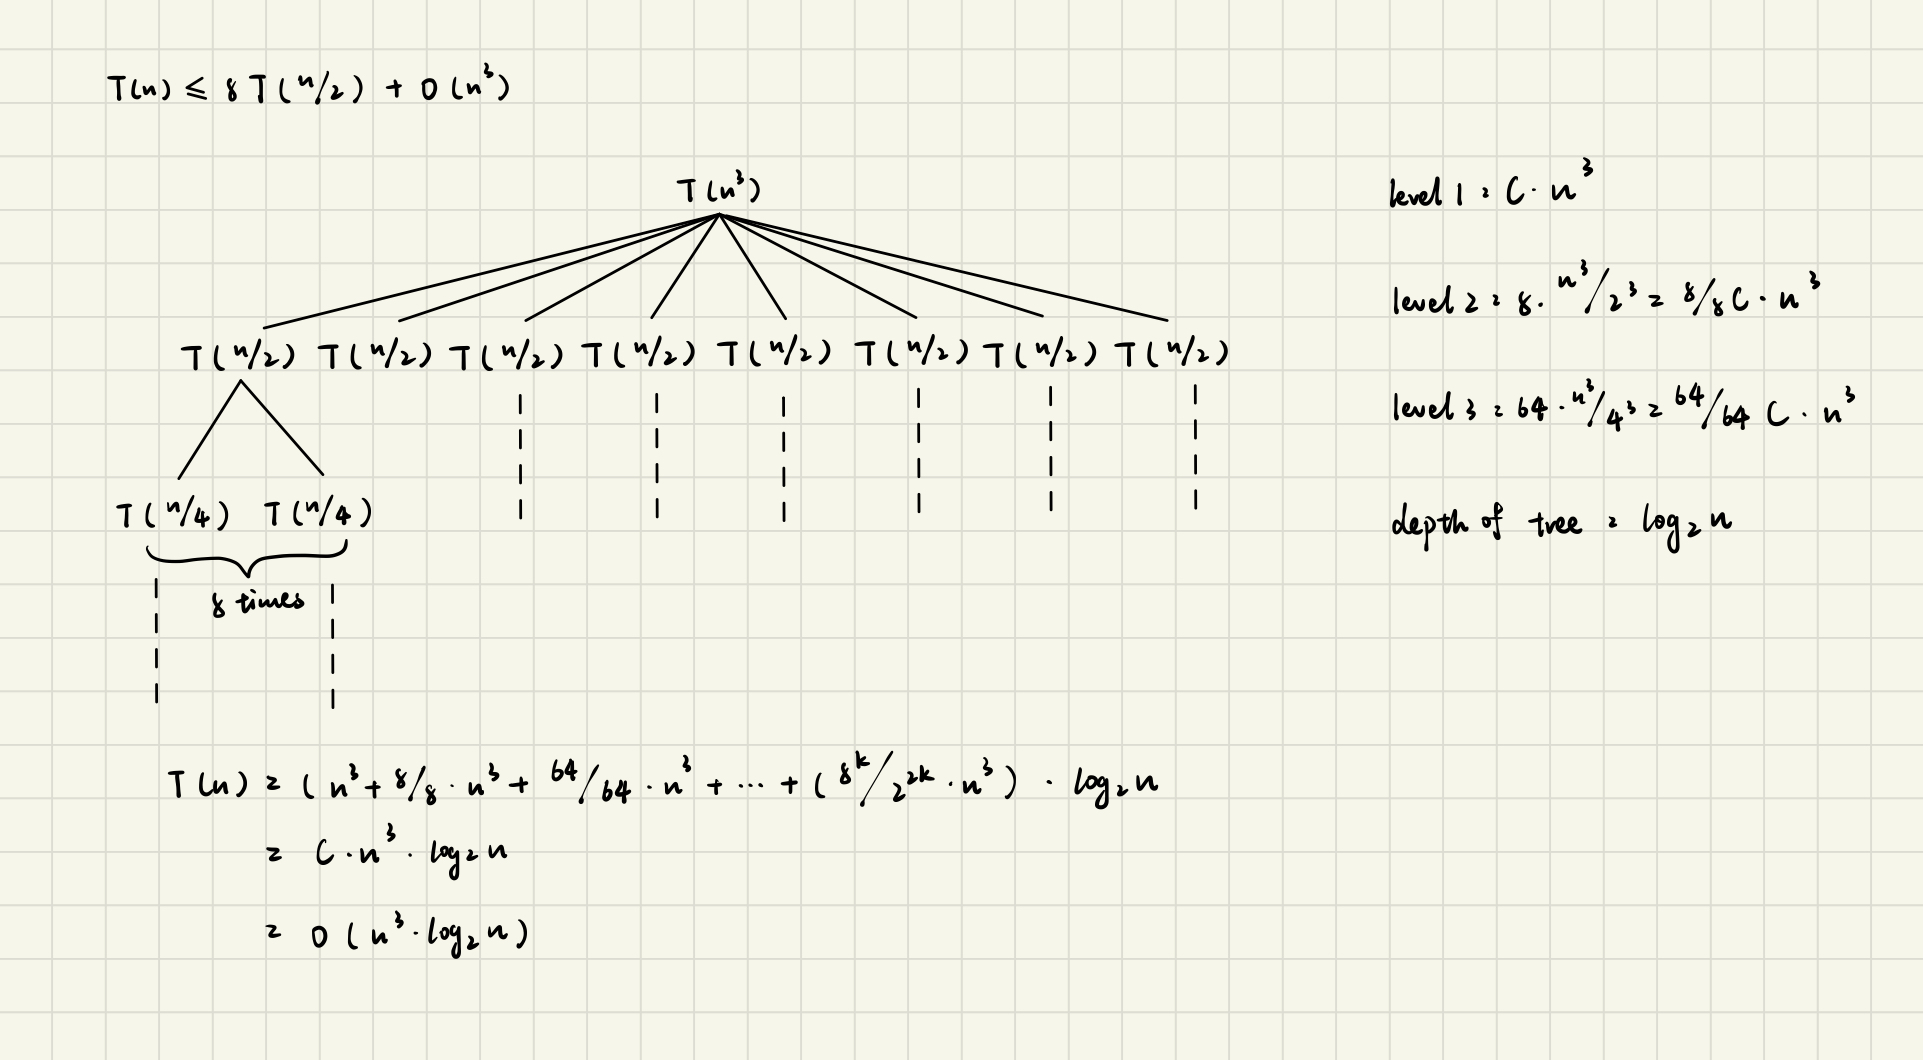
\includegraphics[width=1\textwidth]{midterm.jpg}}{No Figure Yet}
		\caption{Recursion tree for the recurrence in Problem 1-(b).} 
	\end{figure}
	
	Hence, $T(n) = O(n^3\log_2n)$, finalizing the proof.
	
\end{solution}

\end{enumerate}
\end{problem}

\newpage


\begin{problem}\label{induction}
	Consider the algorithm below for finding the total sum of the numbers in any array $A[1:n]$.  
	
	\medskip
	
	$\totalsum (A[1:n])$: \vspace{-0.4cm}
	\medskip
	\begin{enumerate}
		\item If $n=0$: return $0$. 
		\item If $n=1$: return $A[1]$.
		\item Otherwise, let $m_1 \leftarrow \totalsum(A[1:\frac n2])$ and $m_2 \leftarrow \totalsum(A[\frac n2+1:n])$. 
		\item Return  $m_1 + m_2$. 
	\end{enumerate}
	We analyze \totalsum~ in this question. 
	\begin{enumerate}[label=(\alph*)]
		\item Use \emph{induction} to prove the correctness of this algorithm. \grade{10}

\bigskip
	\begin{solution}
	
	\emph{Induction hypothesis:} For any integer n and array A of size n, TOTAL-SUM(A[1 : n]) returns the total sum in the array A, or in other words, returns the correct answer. \\
	
	\emph{Induction base:} For n = 0, there are no element in array A, then the total sum returned should be returned 0. For n = 1, there is only one element in array A, then the total sum should be returned A[1]. By looking the 			algorithm it satisfies both the base cases, thus TOTAL-SUM returns the correct answer in the base case. \\
	
	\emph{Induction step:} Suppose the induction hypothesis is true for all $n > 1$ that n = n + 1. \\
	
	In the case n, if n is even, numbers in array A will be split equally into two calls of TOTAL-SUM(). Conversely, if n is odd, numbers in array A will be split unequally, then the second call of TOTAL-SUM() will have the middle element. 	For any value of n, TOTAL-SUM() will be called until each element of the array is passed to the function as a single-element array input. \\
	
	Furthermore, in the case n = n + 1. If n is odd, adding one becomes even. Numbers in array A will be split equally into two calls of TOTAL-SUM(). Conversely, if n is even, adding one becomes odd. Numbers in array A will be split 	unequally, then the second call of TOTAL-SUM() will have the middle element. \\
	
	Therefore, it is correct for the case n+1. This concludes the proof of induction hypothesis. \\
	
	The correctness of the algorithm now follows directly from the induction hypothesis. \\
		
	\end{solution}


		\newpage
		\item Write a recurrence for this algorithm and solve it to obtain a tight upper bound on the worst case runtime of this algorithm. You can use any method you like for solving this recurrence. 		\grade{10}
	\bigskip	
	
	\begin{solution}
	
	The algorithm is divided into 2 parts of size n/2 for n is even, and is divided into 2 parts of size n/2+1 for n is odd. Plus spends O(1) additional time for getting the results from two subproblems. Hence, if we define T(n) to be the 		worst case runtime of the algorithm on any array of length n, we have $T(n) \leq 2*T(n / 2) + O(1)$.
	
	To solve this recurrence, we first change O(1) with constant c and have $T(n) \leq 2*T(n / 2) + c$. Then, 
	
	%--------
	% If you place a "tree-2-b.pdf" file containing the figure to your recursion tree, it will be shown here. If you like to insert your tree any other way, or do not like to draw one at all, please delete all this line of code below. 
	%--------
	\begin{figure}[h!]
			\centering
			\IfFileExists{midterm2.jpg}{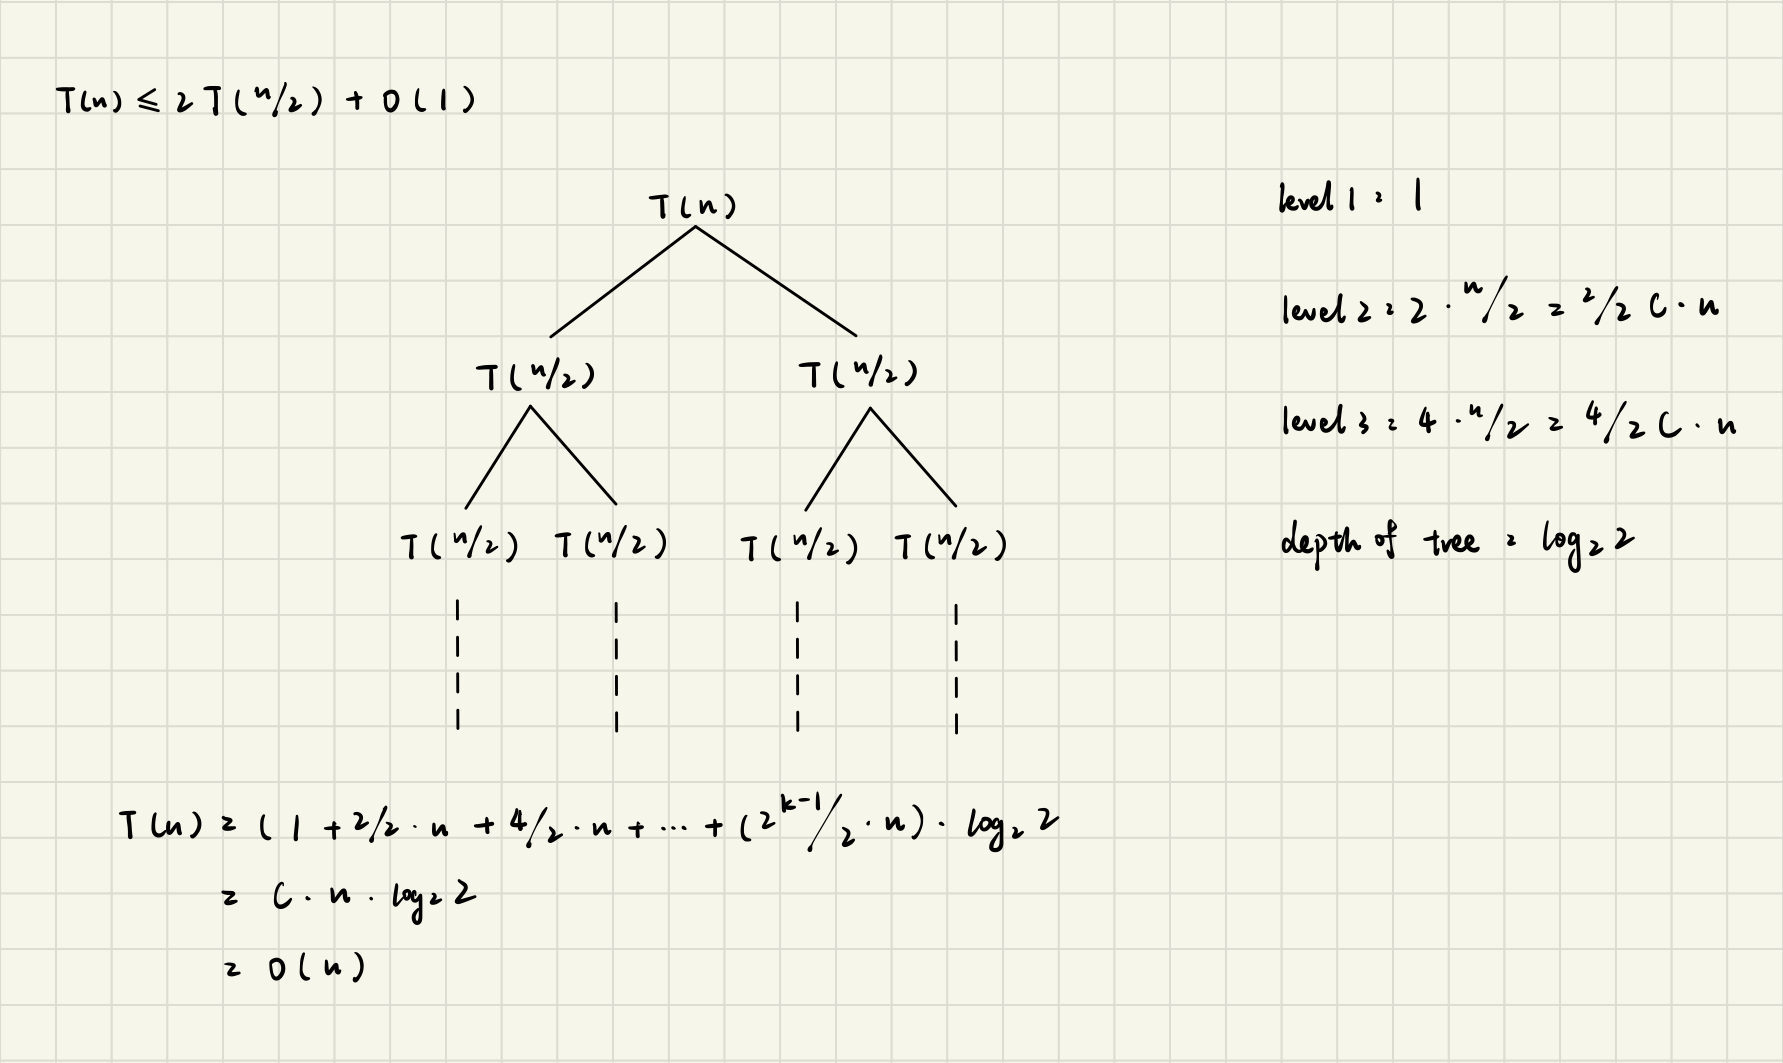
\includegraphics[width=0.8\textwidth]{midterm2.jpg}}{No Figure Yet}
		\caption{Recursion tree for the algorithm in Problem 2-(b).} 
	\end{figure}
	
	Hence, $T(n) = O(n)$ and thus the runtime of this algorithm is O(n). \\
	
\end{solution}


	\end{enumerate}
\end{problem} 

\newpage

\begin{problem}\label{sort}
	You are given a collection of $n$ integers $a_1,\ldots,a_n$ with positive weights $w_1,\ldots,w_n$. For any number $a_i$, we define the \emph{bias} of $a_i$ as:
	\[
		bias(a_i) = |\hspace{-0.1cm}{\sum_{j: a_j < a_i} w_j} - \sum_{k: a_k \geq a_i} w_k|;
	\]
	i.e., the absolute value of the difference between the weights of elements smaller than $a_i$ and the remaining ones. 
	Design and analyze an algorithm that in $O(n\log{n})$ time 
	finds the element that has the \emph{smallest} bias. You can assume that the input is given in two arrays $A[1:n]$ and $W[1:n]$ where $a_i = A[i]$ and $w_i = W[i]$.  

	
	\paragraph{Examples:} 
	\begin{itemize}
	\item When $n=5$, and $A = [1,5,3,2,7]$ and $W=[3,6,2,8,9]$, the smallest biased element is $a_2 = A[2] = 5$ with $bias(a_2) = |(3+2+8)-(6+9)| = 2$.   
	\item When $n=5$, and $A = [1,2,3,4,5]$ and $W=[8,6,5,2,6]$, the smallest biased element is $a_3 = A[3] = 3$ with $bias(a_3) = |(8+6)-(5+2+6)| = 1$. 
	\end{itemize}
	
	\begin{enumerate}[label=(\alph*)]
		\item \emph{Algorithm:} \grade{7}
	
	\bigskip	
	\begin{solution}
	
	(a) Create a combined array B, which contains the elements of array A and array W. \\

	(b) Sort the array B in ascending order according to the first element A[i]. \\
	
	(c) Calculate and store the sum of all the weights in Sum. Let total weight in array A in aWeight. Let total weight in array W in wSum. \\
	
	(d) Traverse array A, for every element in A[i], Initialize $w_j = 0$, $w_k = 0$. \\
	
	(e) For each element in A[j] with A[i]: 	(1) If i = j, then skip the element. 	(2) If $A[j] < A[i]$, adding weight of A[i] to $w_j$. 	(3) If $A[j] > A[i]$, adding weight of A[i] to $w_k$. 	(4) Calculate bias of $A[i], bias = |w_j - w_k|$. 	(5) 	Compare both bias value and let minBias = bias[i].	(6)wSum = Sum - aWeight. 	(6) aWeight = aWeight + W[i]. \\
	
	(f) Output the $minBias$. \\
	
	\end{solution}
	
		\newpage
		\item \emph{Proof of Correctness:} \grade{10}
		
		\bigskip	
	\begin{solution}
	
	Sort the numbers $a_1..a_n$ and their weights in the increasing order of numbers. Hence, to count how many times the number A[i] appears in the array A, we only need to consider the entries in the immediate neighborhood of A 	as is done in the algorithm. More precisely, the value of minBias right before it gets reset for calculating the bias for current element. . Since minBias is simply maintaining the maximum value of Sum throughout the algorithm, we 	obtain that the final answer is correct. 
	
	\end{solution}
	
	
		\item \emph{Runtime Analysis:} \grade{3}
		
		\bigskip	
		
		
	\begin{solution}
	
	The algorithm involves running sort in $O(n log n)$ time and then a for-loop with each iteration taking O(n) time. As such, the total runtime is $O(n log n)$.
	
	\end{solution}
	
		
	\end{enumerate}
\end{problem}
\newpage

\begin{problem}\label{hash}
	You are given three arrays $A[1:n]$, $B[1:n]$, and $C[1:n]$ of positive integers. The goal is to decide whether or not there are indices $i,j,k \in [1:n]$ such that $A[i] \cdot B[j] = C[k]$; in other words, is it the case that there are numbers in $A$ and $B$ whose multiplication belongs to $C$. 
	
	
	\paragraph{Examples:} 
	\begin{itemize}
		\item When $n=3$, and $A = [1,3,4]$, $B=[2,3,5]$, and $C=[1,3,5]$, the answer is \emph{Yes}, because for instance we have $A[1] \cdot B[3] = C[3]$ or $A[1] \cdot B[2] = C[2]$. 
		\item When $n=3$ and $A = [1,3,4]$, $B=[2,4,6]$, and $C=[7,9,11]$, the answer is \emph{No}. 
	\end{itemize} 
	
	\begin{enumerate}[label=$(\alph*)$]
	\item Suppose all the numbers in $C$ belong to the set $\set{1,2,\ldots, n^2}$. Design and analyze an algorithm with \textbf{worst-case runtime} of $O(n^2)$ for the problem in this case. \grade{10} 
	\bigskip	
	\begin{solution} The solution consists of three parts, algorithm, proof of correctness, and runtime analysis. \\
	
	\emph{Algorithm:} The algorithm is as follows: 
	
	(a) Traverse all elements in array C and store it in hash table. \\
	(b) Traverse all elements in array A and array B using for loop, for each element in A takes its product with every element of array B. \\
	(c) Search product in hash table, if matches return \emph{Yes}. \\
	(d) Else return \emph{No}. \\
	
	\emph{Proof of correctness:} The elements of C contain all numbers in ${1, . . . , n^2}$. After multiplying elements in array A and array B, we will. get $C[k] = A[i] \cdot B[j]$. We traverse over A[1 : n] and B[1 : n]for each i, compute 	C(A[i]*B[i]), let C[i] = C(A[i]*B[i]. We obtain that the algorithm outputs j which is the correct answer to the problem.
	
	\emph{Runtime analysis:} Since we traverse all elements in array A and array B using two for loop, the worst case complexity will be $O(n^2)$. Plus for searching product in hash table will take O(1). So, overall the runtime of the 	algorithm is $O(n^2)$ as desired.
	
	\end{solution}
	
	
	\newpage
	\item Now suppose $C$ can be any arbitrary array of $n$ integers. Design and analyze a \textbf{randomized} algorithm with \textbf{expected worst-case runtime} of $O(n^2)$ for the problem in this case. \grade{10} 

	\medskip
	\emph{Note:} Actually, this problem also has a deterministic algorithm that runs in worst-case $O(n^2)$ time. But you do not need to design such an algorithm for this problem (although if you do, you will receive the full credit for both parts $(a)$ and $(b)$).
	
	\bigskip	
	\begin{solution} The solution consists of three parts, algorithm, proof of correctness, and runtime analysis. \\
	
	\emph{Algorithm:} The algorithm is as follows: 
	
	(a) Create a hash table T of size m = n using a near-universal random hash family, and by handling collisions using the chaining method. \\
	(b) Insert all elements of C into the hash table T. \\
	(c) Traverse all elements in array A and array B using for loop, for each element in A takes its product with every element of array B. \\
	(d) Search product in hash table, if matches return \emph{Yes}. \\
	(e) Else return \emph{No}. \\
	
	\emph{Proof of correctness:} By correctness of hash table T , we know that every element of C that is hashed to T will be found via search operation. After multiplying elements in array A and array B, we will. get $C[k] = A[i] \cdot B[j]$. We traverse over A[1 : n] and B[1 : n]for each i, compute 	C(A[i]*B[i]), let C[i] = C(A[i]*B[i]. We obtain that the algorithm outputs j which is the correct answer to the problem.
	
	\emph{Runtime analysis:} Since we traverse all elements in array A and array B using two for loop, the worst case complexity will be $O(n^2)$. Plus for searching product in hash table will take O(1). So, overall the runtime of the 	algorithm is $O(n^2)$ as desired.

	
	
	\end{solution}
	
	
	\end{enumerate}
	
	
\end{problem}

\newpage
\begin{problem}\label{DP-greedy}
Please solve the problems in \textbf{exactly one} of the two parts below. 

\paragraph{Part 1 (dynamic programming):} We want to purchase an item of price $M$ and for that we have a collection of $n$ different coins in an array $C[1:n]$ where coin $i$ has value $C[i]$ (we only have one copy of each coin).  
	Our goal is to purchase this item using the \emph{smallest} possible number of coins or outputting that the item cannot be purchased with these coins. 
	Design a \textbf{dynamic programming} algorithm for this problem with worst-case runtime of $O(n \cdot M)$. \grade{20}
	
	\paragraph{Examples:}
	\begin{itemize}
		\item Given $M=15$, $n=7$, and $C = [4,9,3,2,7,5,6]$, the correct answer is $2$ by picking $C[2]=9$ and $C[7]=6$ which add up to $15$. 
		\item Given $M=11$, $n=4$, and $C = [4,3,5,9]$, the correct answer is that `the item cannot be purchased' as no combination of these coins adds up to a value of $11$ (recall that we can only use each coin once). 
	\end{itemize}
	
	\begin{enumerate}[label=(\alph*)]
	\item \emph{Specification of recursive formula for the problem (in plain English)}: \grade{5}
	
	\bigskip	
	\begin{solution}
	
	For any integer $0\leq i \leq M$, we define: \\

	• V(i): the the minimum number of coins required to have a total value of M. If there is no combination of these coins we output ‘the item cannot be purchased’. \\
	
	The solution to the problem can be obtained by returning V(n). \\
	
	\end{solution}
	
	
	\item \emph{Recursive solution for the formula and its proof of correctness:} \grade{7}
	
	\bigskip	
	\begin{solution}

	The recursive formula for V(i) is as follows: 
	
	\begin{align*}
 		\begin{split}
 			V(i)= \left \{
 			\begin{array}{ll}
 				0,                      				& if  i = n\\
 				C[i],     					& if  i > n\\
 				min({V(i_1) + V(i_2)}),                  & otherwise
 			\end{array}
		\right.
 		\end{split}
	\end{align*}
		
	\emph{Proof of Correctness:} We consider each case separately: \\
	• If i = 0, the item cannot be purchased and thus V(0)=0 is the correct value. \\
	• If i > 1, since all items, and in particular item A[1] has a positive value, we can and should pick A[1] which makes V(1) = C[i]. \\
	• Otherwise, we have two options: (1) we do not use any coins i: in this case, no combination of these coins adds up to a value of M (recall that we can only use each coin once). (2) we pick item i: in this case, we will gain the value 	of $V_i$ but no longer can pick item i as otherwise we will have two consecutive items in the solution which is not possible; thus, in this case, we should skip over item M and pick the best solution from {1,...,M} captured by $V(i_2)$ 	(since $i \geq M$,  and thus $V(i_1) + V(i_2)$ is well defined). \\
	Consequently, in option (1) we get the value of $V_i$ (just from the items we pick from {1,...,M}) and in option (2) we get the value of $V(i_1)+V(i_2)$ (from the items we pick from {1, . . . , M} and the item i that we picked). Since our 	goal is to find the maximum value possible, taking the max of the two options, as done by the formula, ensures the correctness.
	
	
	\end{solution}
	
	
	\newpage
	\item \emph{Algorithm (either memoization or bottom-up dynamic programming):} \grade{3}
	
	\bigskip	
	\begin{solution}
	
	We design a memoization algorithm for the problem. \\
	Let T [1 : n] be an n dimensional array originally filled with ‘undefined’. We write the following recursive function:
	memV(i) :
	(1) If i = 0, return 0;
	(2) If i = 1, return vi;
	(3) If T [i] = |undefined’ return T [i].
	(4) Else let $T[i] = minBias$. 
	(5) Return T[i]. \\
	The answer to the problem can then be computed. \\
	
	\end{solution}
	
	\item \emph{Runtime Analysis:} \grade{5}
	
	\bigskip	
	\begin{solution}
	
	There are n + 1 = O(n) subproblems for the recursive formula V(). Moreover, each subproblem takes O(1) to compute, hence the total runtime of the algorithm is O(n) as desired.
	
	\end{solution}
	
	
\end{enumerate}


\newpage
\paragraph{Part 2 (greedy):} 
	We want to purchase an item of price $M$ and for that we have an unlimited (!) supply of $\ceil{\log{M}}$ types of coins with value $1,2,4,\cdots,2^{i},\cdots,2^{\ceil{\log{M}}}$. 
	Our goal is to purchase this item using the \emph{smallest} possible number of coins (it is always possible to buy this item by picking $M$ coins of value $1$).
	Design and analyze a \textbf{greedy} algorithm for this problem with $O(\log{M})$ runtime. \grade{20}

	\paragraph{Examples:} 
	\begin{itemize}
		\item Given $M=15$ (and so $\ceil{\log{M}} = 4$), the correct answer is $4$ coins by picking one copy of each of the coins $8,4,2,1$. Note that here we cannot pick the coin of value $2^{\ceil{\log{M}}} = 2^{4} = 16$.
		\item Given $M=32$ (and so $\ceil{\log{M}} = 5$), the correct answer is $1$ coin by picking one copy of the coin $32 = 2^{5} = 2^{\ceil{\log{M}}}$. 

	\end{itemize}
		
		\begin{enumerate}[label=(\alph*)]
	\item \emph{Algorithm}: \grade{5}
	
	\bigskip
				\begin{solution}
	Solution to part (a) goes here. 
	\end{solution}
	
	
	\newpage
	\item \emph{Proof of Correctness}: \grade{10}
	\bigskip
				\begin{solution}
	Solution to part (b) goes here. 
	\end{solution}
	
	\bigskip
	
	\item \emph{Runtime Analysis:} \grade{5}
	\bigskip
				\begin{solution}
	Solution to part (c) goes here. 
	\end{solution}
	
	
\end{enumerate}

\end{problem}
\newpage

\begin{problem}\label{extra}[\textbf{Extra credit}]
	You are given two \emph{unsorted} arrays $A[1:n]$ and $B[1:n]$ consisting of $2n$ \emph{distinct} numbers such that $A[1] < B[1]$ but $A[n] > B[n]$. Design and analyze an algorithm that in $O(\log{n})$ time 
	finds an index $j \in [1:n]$ such that $A[j] < B[j]$ but $A[j+1] > B[j+1]$. 
	
	\emph{Hint:} Start by convincing yourself that such an index $j$ always exist in the first place. \grade{+10}

\end{problem}

\bigskip

	\begin{solution}

	\emph{Algorithm:} (a) Traverse and sort array B. (b) Traverse array A. (c) Run a binary search on array B and find the index of the largest element smaller than the element of array A. \\
	
	\emph{Proof of Correctness:} We know that the arrays are consisting of 2n distinct numbers such that $A[1] < B[1]$ but $A[n] > B[n]$. \\
	
	\emph{Runtime Analysis:} The worst-case runtime of the algorithm is $O(m\log{n} + n\log{n})$.
	
	\end{solution}
	
\newpage
\subsection*{Extra Workspace}


\end{document}





